\documentclass{beamer}

%Preamble
\title{Latex Slides}
\author{Amanpreet Singh}
\date{Oct 25, 2023}
\usetheme{CambridgeUS}
\usecolortheme{crane}

%Config
\graphicspath{{../../../../../common/images/stock/}}

\begin{document}
\maketitle

\begin{frame}
\frametitle{First Slide}
This is first Slide created with Latex and Beamer.\\
This has just the Normal Text.

Following \href{https://latex-beamer.com/tutorials/beamer-themes/}{Tutorial} for Basics of Latex and Beamer.
\end{frame}

\begin{frame}
\frametitle{Themes}
Beamer has many \textbf{Themes} which can be specified in preamble.

\textbf{Theme Sources}
\begin{itemize}
    \item \href{https://deic.uab.cat/~iblanes/beamer_gallery/index_by_theme.html}{Theme Browser}
    \item \href{https://hartwork.org/beamer-theme-matrix/}{Theme Matrix} (Theme and Color)
\end{itemize}

\end{frame}

\begin{frame}
    \frametitle{Formatting}
    List Heading
    \begin{itemize}
        \item Content of this Slide.
        \item In Bullet Point format.
        \item It is very easy to Create.
        \item Wait before Next Section.\pause
    \end{itemize}

    \begin{alertblock}{Warning}
        Alert message in Alert Block !!
    \end{alertblock}

    \begin{exampleblock}{Example}
        Example message in Example Block ..
    \end{exampleblock}

\end{frame}

\begin{frame}
    \frametitle{Images}
    A Sail Boat ..
    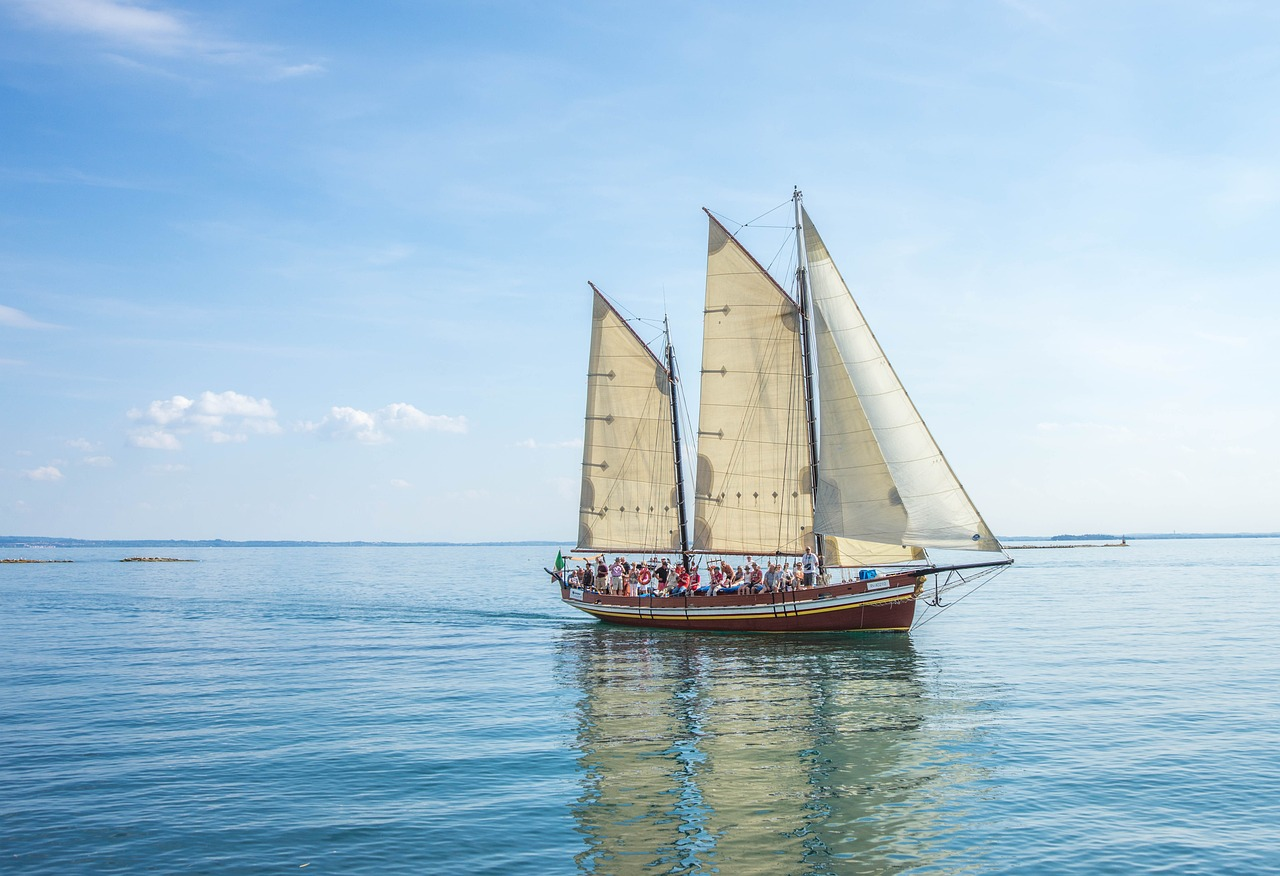
\includegraphics[width=0.8\linewidth]{boat.jpg}
\end{frame}

\end{document}